\documentclass[12pt]{article}
\usepackage{times} 			% use Times New Roman font

\usepackage[margin=1in]{geometry}   % sets 1 inch margins on all sides
\usepackage[hidelinks]{hyperref}               % for URL formatting
\usepackage[pdftex]{graphicx}       % So includegraphics will work
\setlength{\parskip}{1em}           % skip 1em between paragraphs
\usepackage{indentfirst}            % indent the first line of each paragraph
\usepackage{datetime}
\usepackage[small, bf]{caption}
\usepackage{listings}               % for code listings
\usepackage{xcolor}                 % for styling code
\usepackage{multirow}
\usepackage{subcaption}     % for subfigures

%\setlength\intextsep{1.69cm} 

%New colors defined below
\definecolor{backcolour}{RGB}{246, 246, 246}   % 0xF6, 0xF6, 0xF6
\definecolor{codegreen}{RGB}{16, 124, 2}       % 0x10, 0x7C, 0x02
\definecolor{codepurple}{RGB}{170, 0, 217}     % 0xAA, 0x00, 0xD9
\definecolor{codered}{RGB}{154, 0, 18}         % 0x9A, 0x00, 0x12

%Code listing style named "gcolabstyle" - matches Google Colab
\lstdefinestyle{gcolabstyle}{
  basicstyle=\ttfamily\small,
  backgroundcolor=\color{backcolour},   
  commentstyle=\itshape\color{codegreen},
  keywordstyle=\color{codepurple},
  stringstyle=\color{codered},
  numberstyle=\ttfamily\footnotesize\color{darkgray}, 
  breakatwhitespace=false,         
  breaklines=true,                 
  captionpos=b,                    
  keepspaces=true,                 
  numbers=left,                    
  numbersep=5pt,                  
  showspaces=false,                
  showstringspaces=false,
  showtabs=false,                  
  tabsize=2
}

\lstset{style=gcolabstyle}      %set gcolabstyle code listing

% to make long URIs break nicely
\makeatletter
\g@addto@macro{\UrlBreaks}{\UrlOrds}
\makeatother

% for fancy page headings
\usepackage{fancyhdr}
\setlength{\headheight}{13.6pt} % to remove fancyhdr warning
\pagestyle{fancy}
\fancyhf{}
\rhead{\small \thepage}
\lhead{\small HW1\, Tomar}  % EDIT THIS, REPLACE # with HW number
\chead{\small CS 532, Spring 2023} 

%-------------------------------------------------------------------------
\begin{document}

% EDIT THE ITEMS HERE
\begin{centering}
{\large\textbf{HW1\ - Web Science Intro}}\\ 
Prashant Tomar\\
Jan 29, 2023\\
\end{centering}

%-------------------------------------------------------------------------

% The * after \section just says to not number the sections
\section*{Q1}

\emph{}

\subsection*{Answer}

Figure \ref{fig:Q1a} shows the Directed Graph showing how the nodes are connected to each other.


\begin{figure}[h!]
    \centering
    % trim and clip are used to crop the image, trim=left bottom right top
    % width sets max width, height will be scaled appropriately
    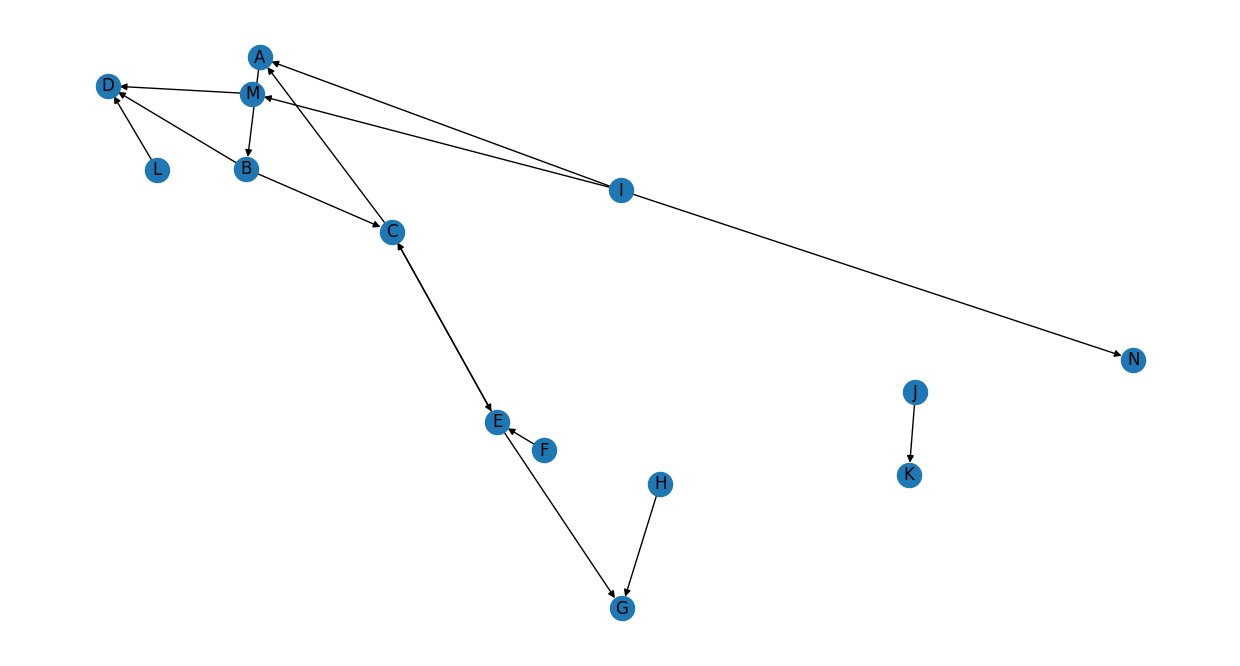
\includegraphics[trim=0 0 0 0, clip, width=\textwidth,height=10cm] {Q1a.png}
    \caption{Directed Graph}
    \label{fig:Q1a}
\end{figure}

Table \ref{tbl:simple} shows a nodes that are listed in the following categories.

\begin{table}[h!]
\centering
\caption{Simple Table}
\label{tbl:simple}
\begin{tabular}{|l|l|l|}
\hline
\textbf{S.No.} & \textbf{Categories} & \textbf{Nodes} \\ \hline \hline
1 & SCC: & A,B,C,E  \\ \hline
2 & IN: & D,G \\ \hline
3 & OUT: & F,H,I,L \\ \hline
4 & Tendrils: & N \\ \hline
5 & Tubes: & M  \\ \hline
6 & Disconnected: & J,K \\ \hline
\end{tabular}
\end{table}



\subsection*{Discussion}

\emph{Tendrils: Pages that cannot reach the SCC and cannot be reached from the SCC.
Pages that can only be reached from IN, or can only reach OUT. In our case, N is only reach OUT.
}

\emph{Tubes: Connects a TENDRIL hanging off from IN to a TENDRIL leading into OUT (a passage from a portion of IN to a portion of OUT without touching SCC). Pages that have in-links from IN or other pages in Tubes and out-links to pages in Tubes or OUT.}

%Importing code from file
\lstinputlisting[language=Python, caption=Python sample code loaded from file, label=lst:import]{abc.py}


\section*{Q2}

(a) First, load the URI directly in your browser and take a screenshot. The resulting webpage should show the "User-Agent" HTTP request header that your web browser sends to the web server. 
Figure \ref{fig:Q2a} Webpage shows the ”User-Agent” HTTP request header that your web browser sends to the web
server.

\begin{figure}[h!]
    \centering
    % trim and clip are used to crop the image, trim=left bottom right top
    % width sets max width, height will be scaled appropriately
    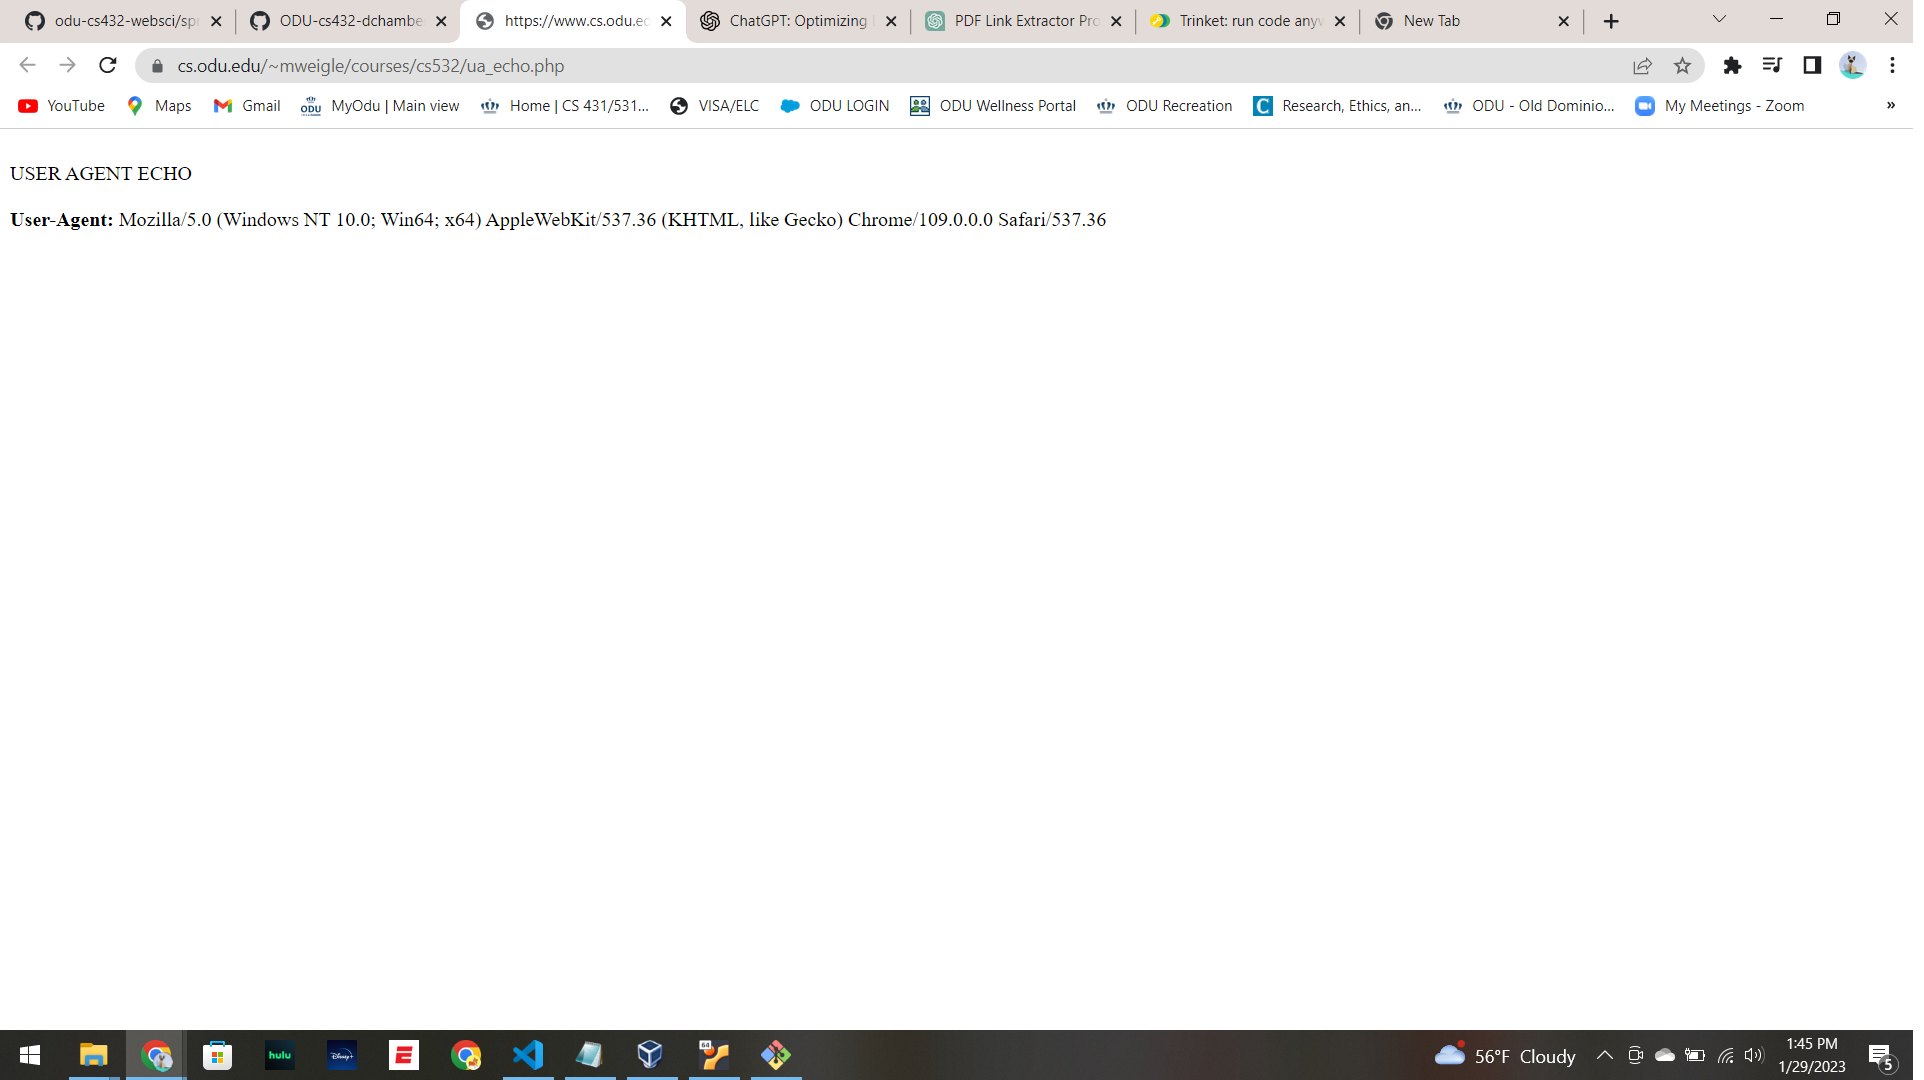
\includegraphics[trim=0 10 20 20, clip, width=\textwidth] {Q2a.png}
    \caption{Webpage shows the ”User-Agent” HTTP request header that your web browser sends to the web server}
    \label{fig:Q2a}
\end{figure}

(b)  In a single curl command, request the URI, show the HTTP response headers, follow any redirects, and change the User-Agent HTTP request field to "CS432/532". Show command you used and the result of your execution on the command line. (Either take a screenshot of your terminal or copy/paste into a code segment.)

%Curl command used
\begin{lstlisting}[language=Python, caption=Python example copied into the LaTeX, label=lst:copy]
> curl -I -L -H "User-Agent: CS432/532" http://www.cs.odu.edu/\~mweigle/courses/cs532/ua_echo.php
\end{lstlisting}

Figure \ref{fig:Q2b} Requested the URI which shows the HTTP response headers, follow any redirects, and changed
User-Agent HTTP request field to ”CS432/532”.

\begin{figure}[h!]
    \centering
    % trim and clip are used to crop the image, trim=left bottom right top
    % width sets max width, height will be scaled appropriately
    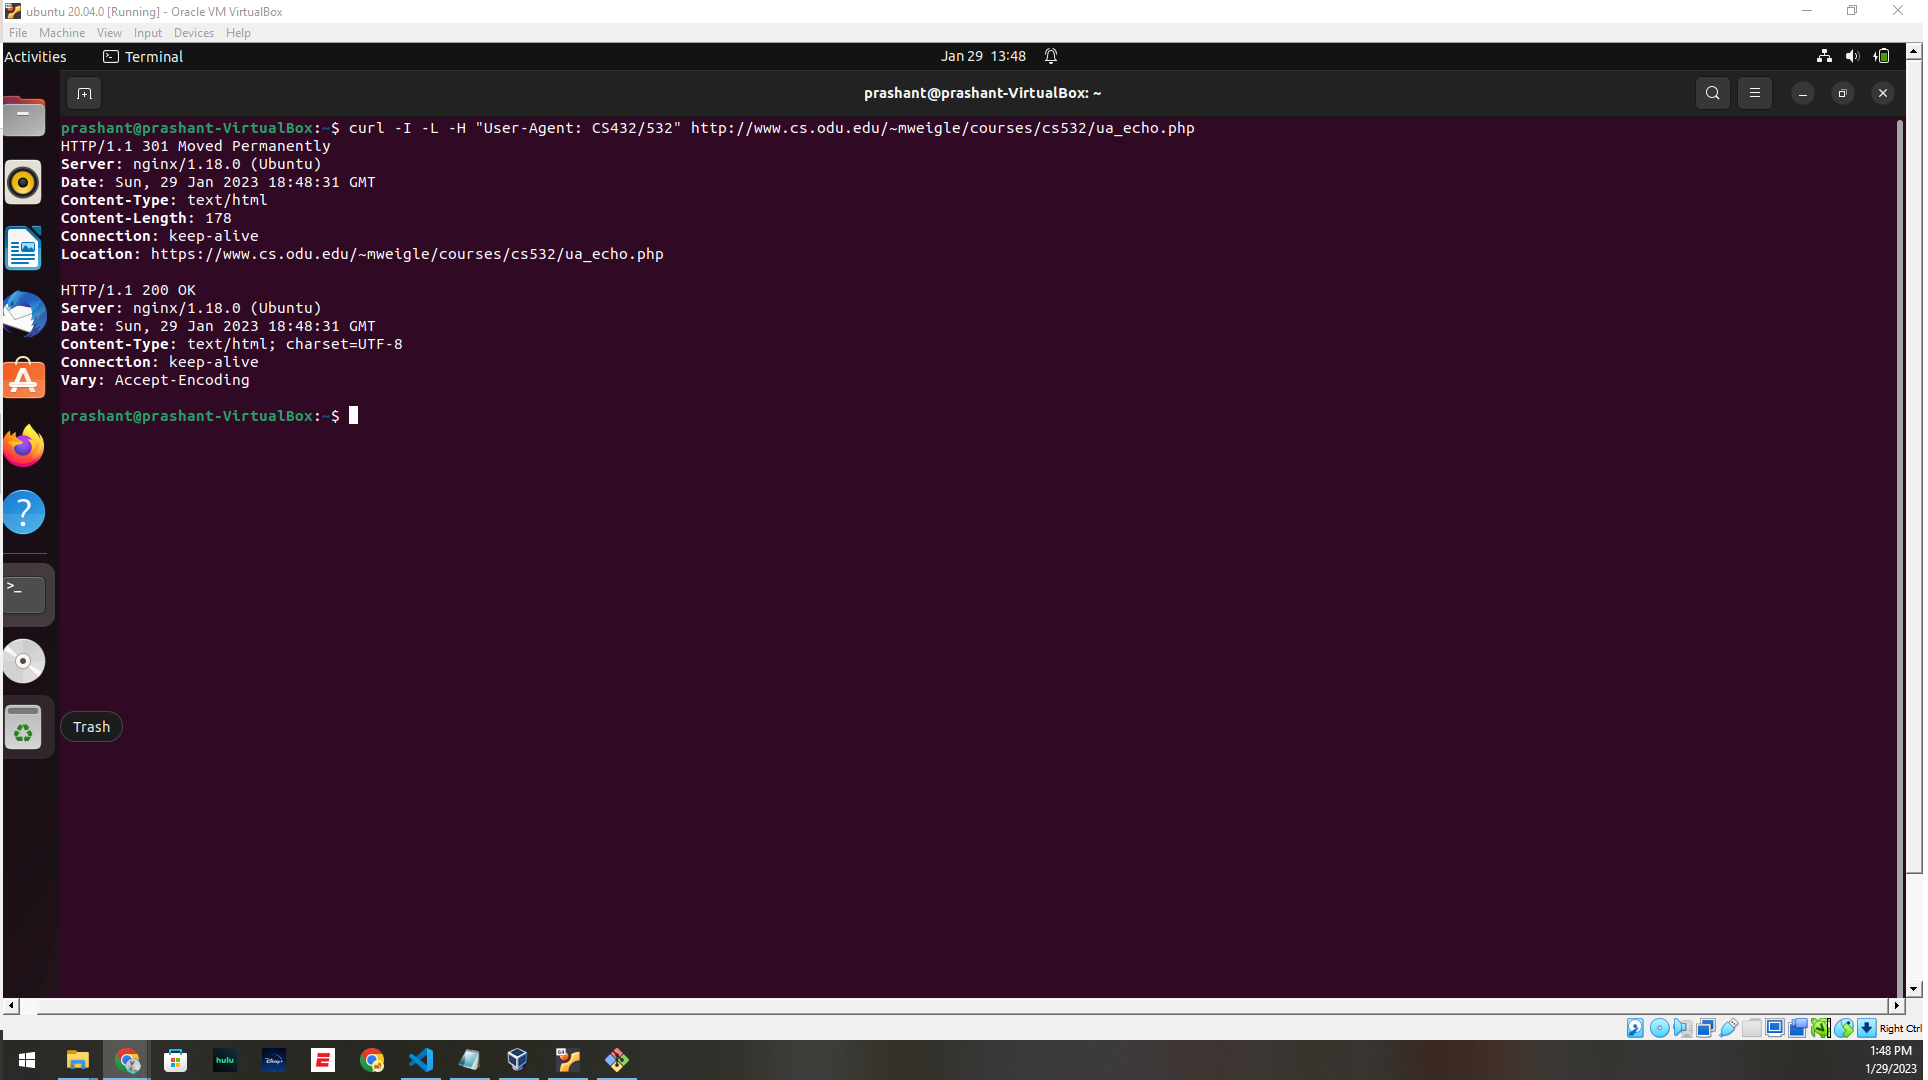
\includegraphics[trim=0 0 0 0, clip, width=\textwidth,height=10cm] {Q2b.png}
    \caption{Requested the URI which shows the HTTP response headers, follow any redirects, and changed User-Agent HTTP request field to "CS432/532".}
    \label{fig:Q2b}
\end{figure}


(c) In a single curl command, request the URI, follow any redirects, change the User-Agent HTTP request field to "CS432/532", and save the HTML output to a file. Show the command you used and the result of your execution on the command line. View the HTML output file that was produced by curl in a web browser and take a screenshot.

%Curl command used
\begin{lstlisting}[language=Python, caption=Python example copied into the LaTeX, label=lst:copy]
> curl -I -L -H "User-Agent: CS432/532" http://www.cs.odu.edu/\~mweigle/courses/cs532/ua_echo.php --output index.html
\end{lstlisting}

Figure \ref{fig:Q2c-1} shows the process of giving path to html file

\begin{figure}[h!]
    \centering
    % trim and clip are used to crop the image, trim=left bottom right top
    % width sets max width, height will be scaled appropriately
    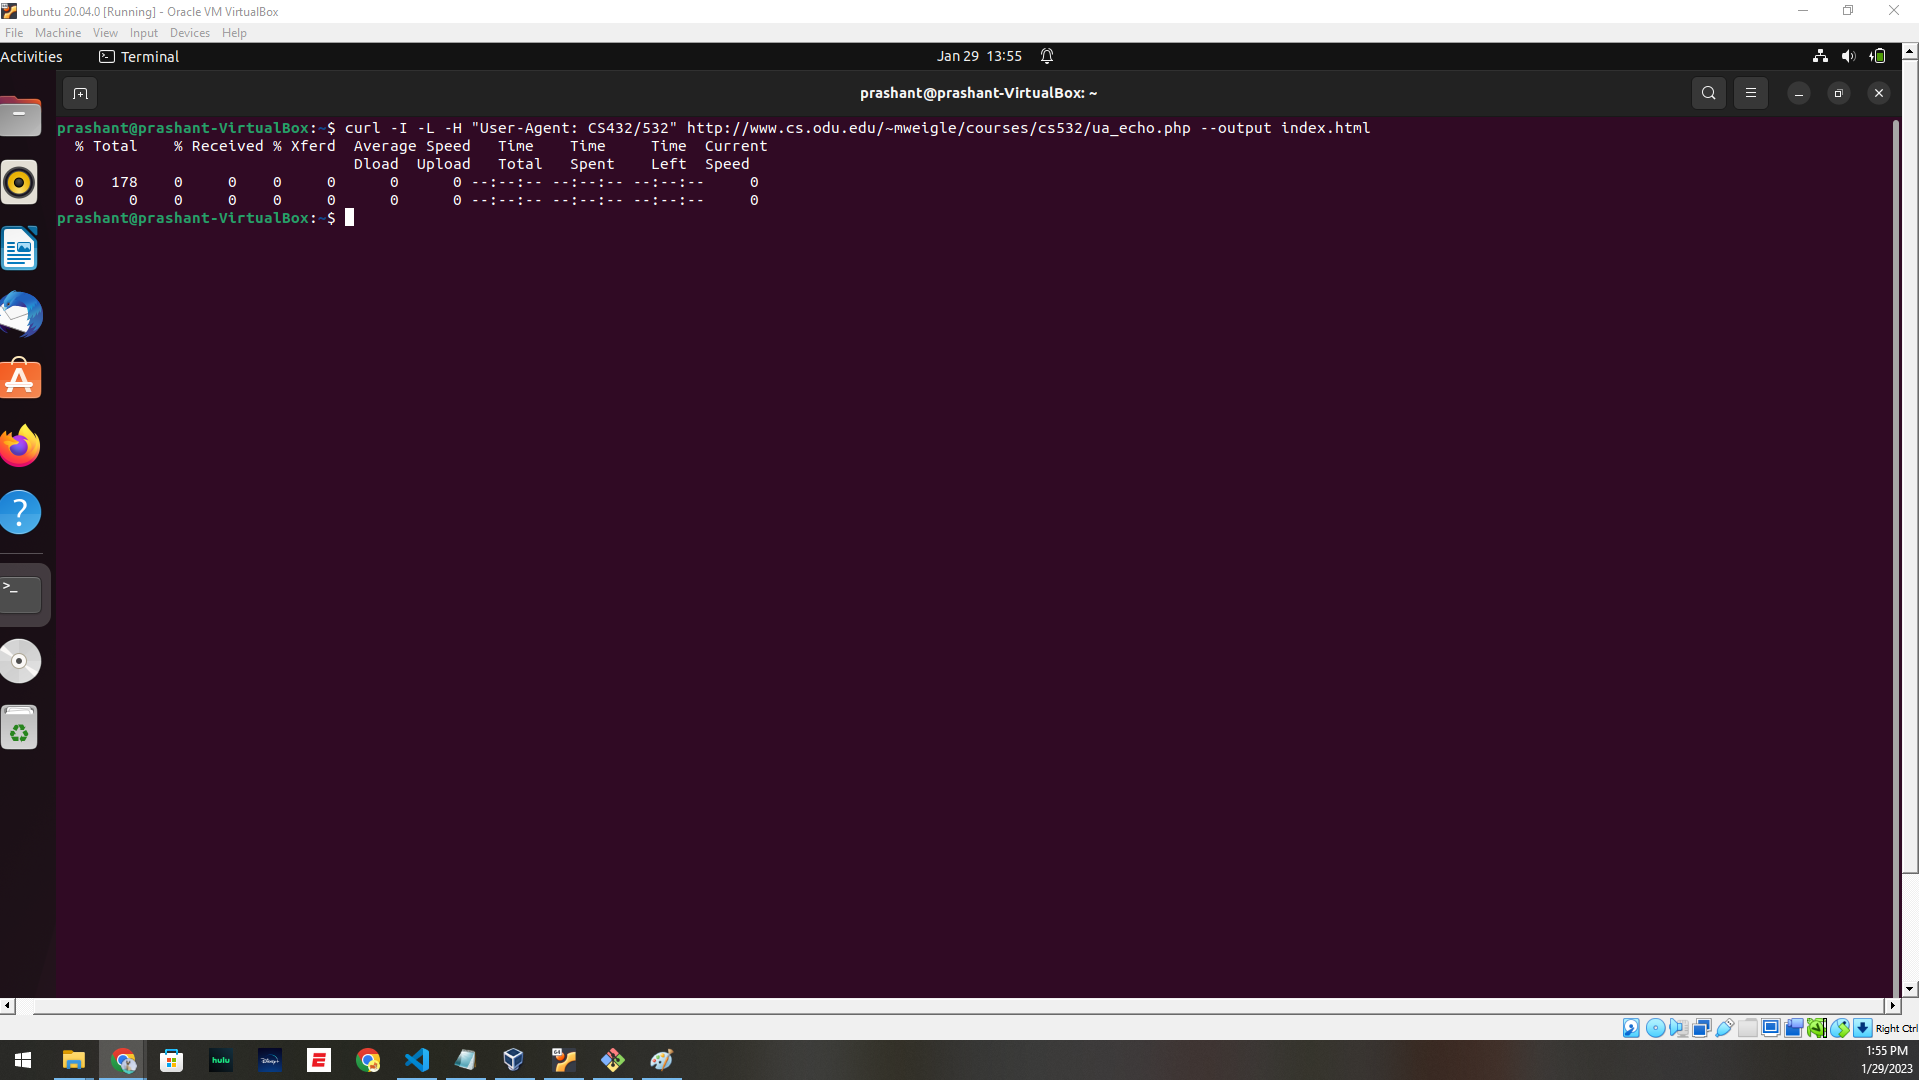
\includegraphics[trim=0 0 0 0, clip, width=\textwidth,height=10cm] {Q2c-1.png}
    \caption{Giving path to html file}
    \label{fig:Q2c-1}
\end{figure}

Figure \ref{fig:Q2c-2} shows the path of HTML file on local machine.

\begin{figure}[h!]
    \centering
    % trim and clip are used to crop the image, trim=left bottom right top
    % width sets max width, height will be scaled appropriately
    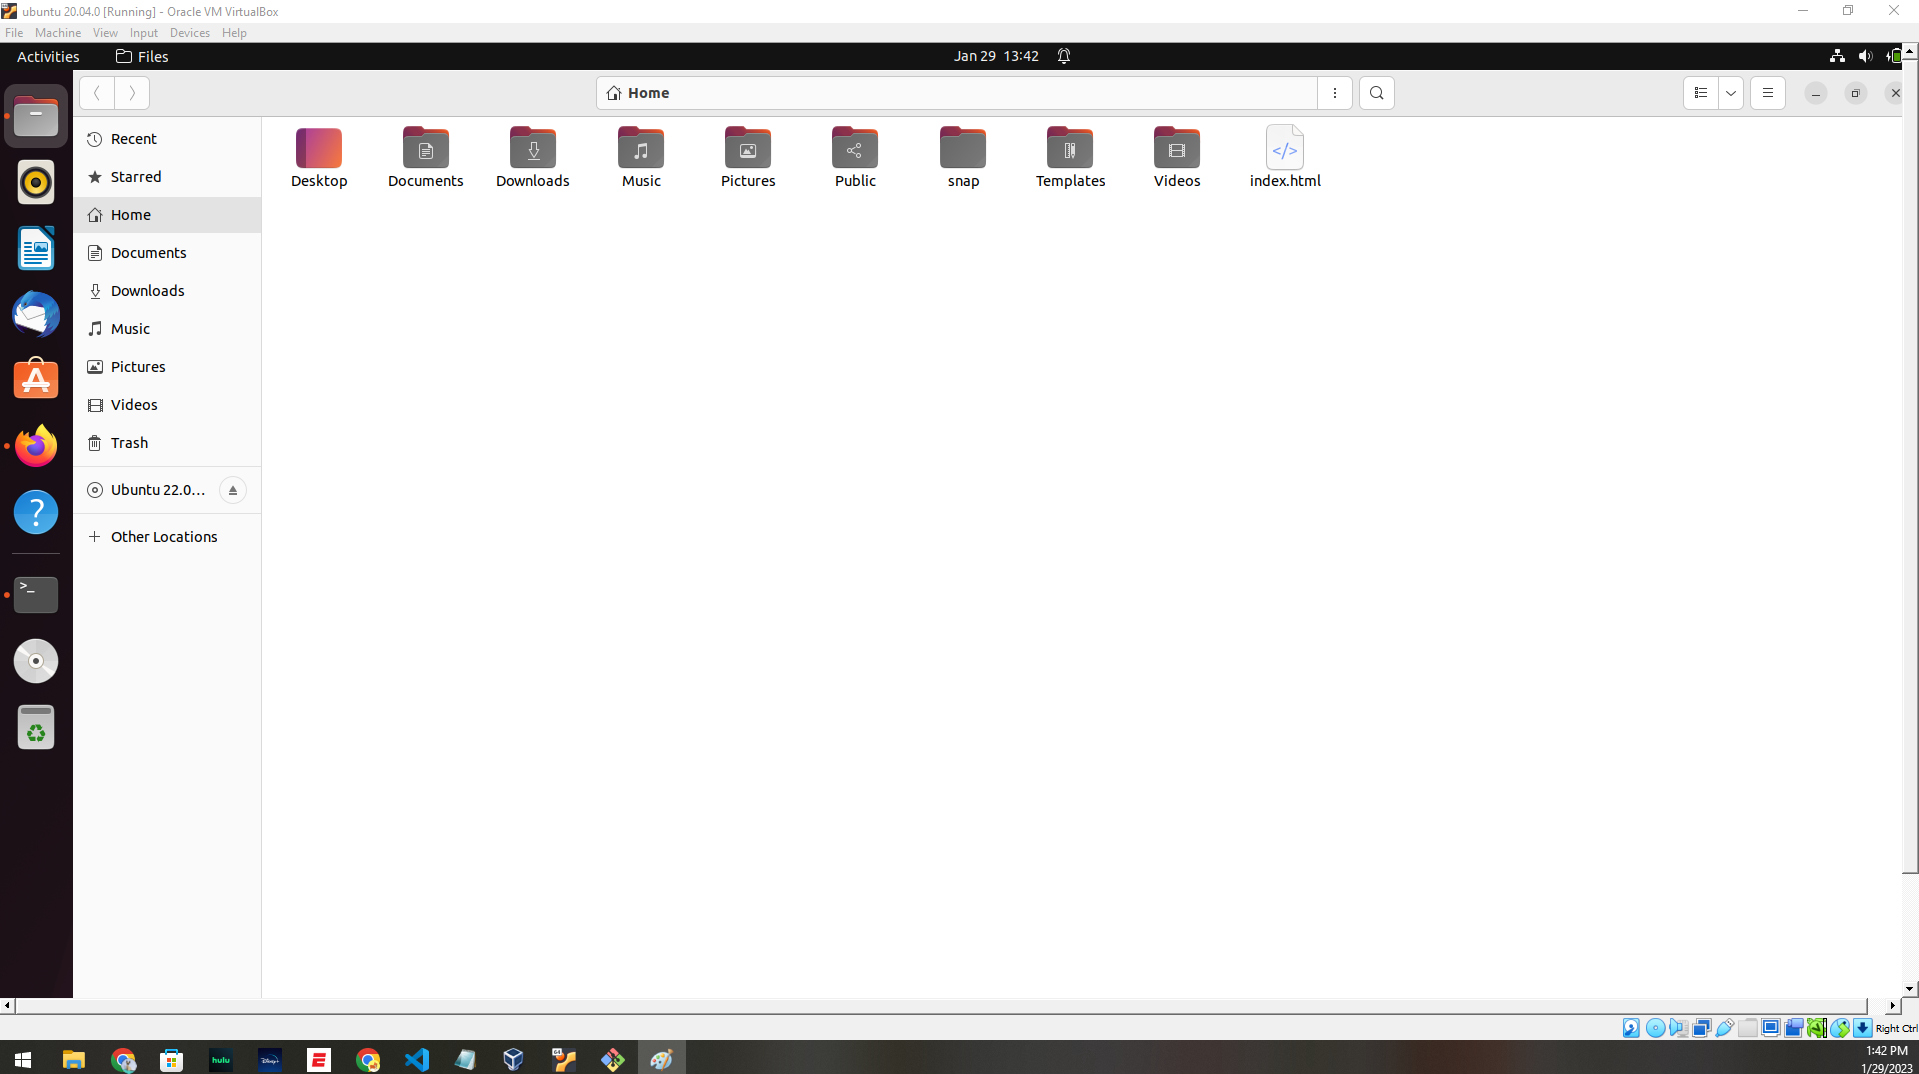
\includegraphics[trim=0 0 0 0, clip, width=\textwidth,height=10cm] {Q2c-2.png}
    \caption{HTML file on local machine}
    \label{fig:Q2c-2}
\end{figure}

Figure \ref{fig:Q2c-3} shows the Requested the URI which follow any redirects and changed the User-Agent HTTP request field to ”CS432/532”, and saved the HTML output to a file.


\begin{figure}[h!]
    \centering
    % trim and clip are used to crop the image, trim=left bottom right top
    % width sets max width, height will be scaled appropriately
    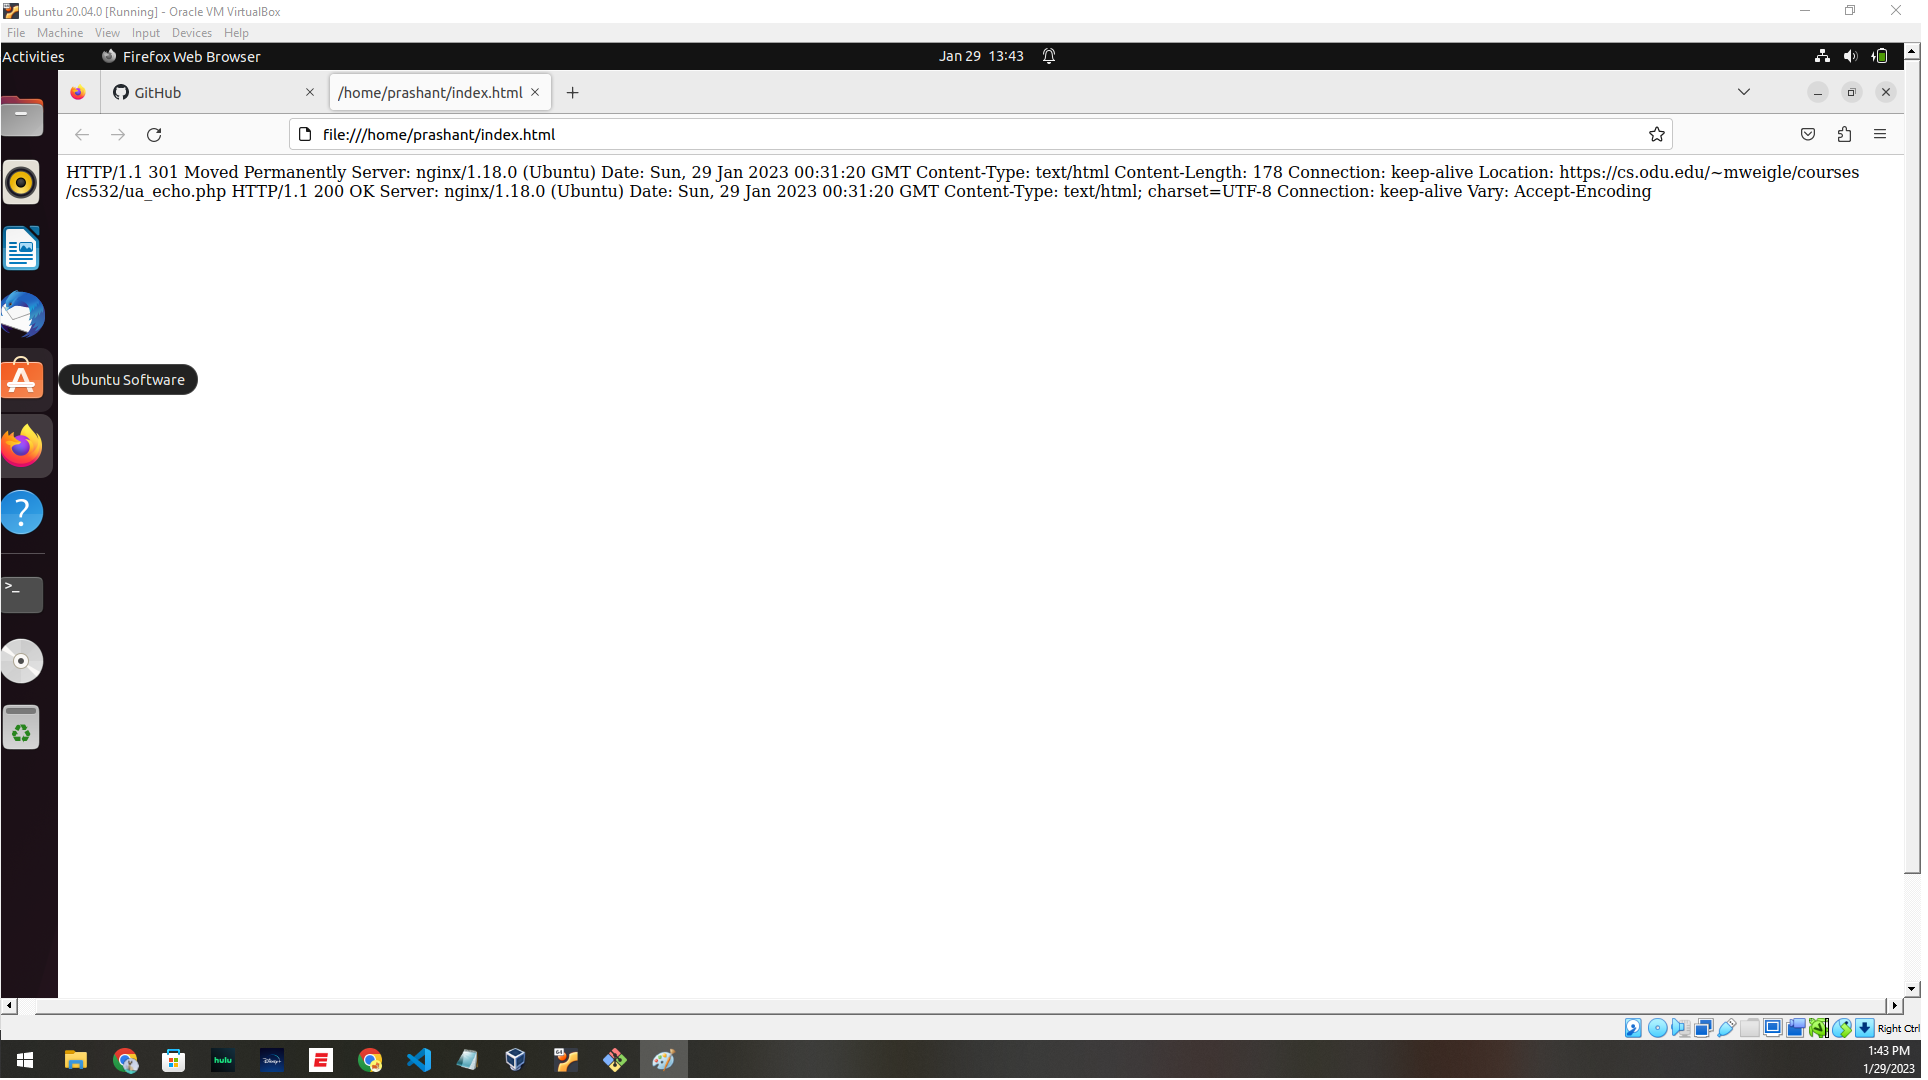
\includegraphics[trim=0 0 0 0, clip, width=\textwidth,height=10cm] {Q2c-3.png}
    \caption{Requested the URI which follow any redirects and changed the User-Agent HTTP request field to "CS432/532", and saved the HTML output to a file.}
    \label{fig:Q2c-3}
\end{figure}

\subsection*{Discussion}

\section*{Q3}

\subsection*{Answer}

\begin{figure}[H]
    \centering
    % trim and clip are used to crop the image, trim=left bottom right top
    % width sets max width, height will be scaled appropriately
    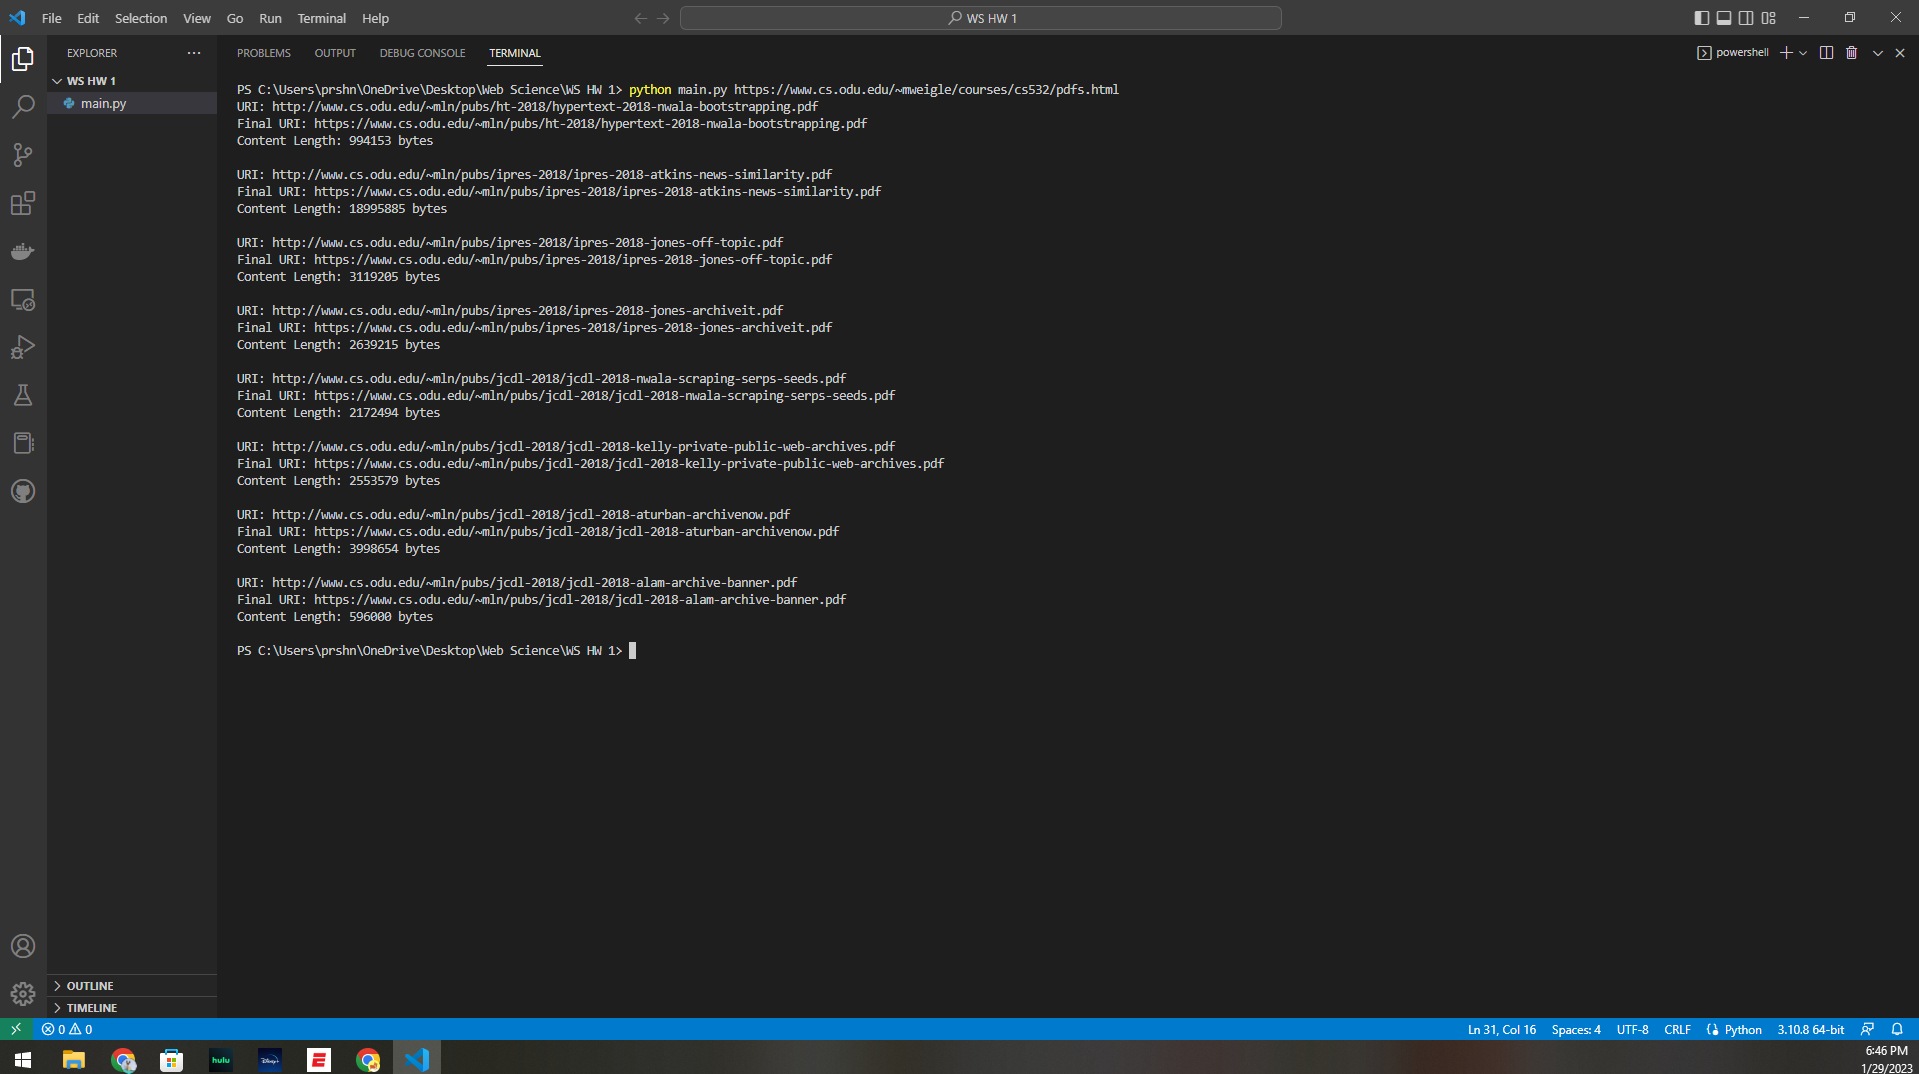
\includegraphics[trim=0 0 0 0, clip, width=\textwidth,height=10cm] {Q3a.png}
    \caption{PDF:1}
    \label{fig:Q3a}
\end{figure}

\begin{figure}[h!]
    \centering
    % trim and clip are used to crop the image, trim=left bottom right top
    % width sets max width, height will be scaled appropriately
    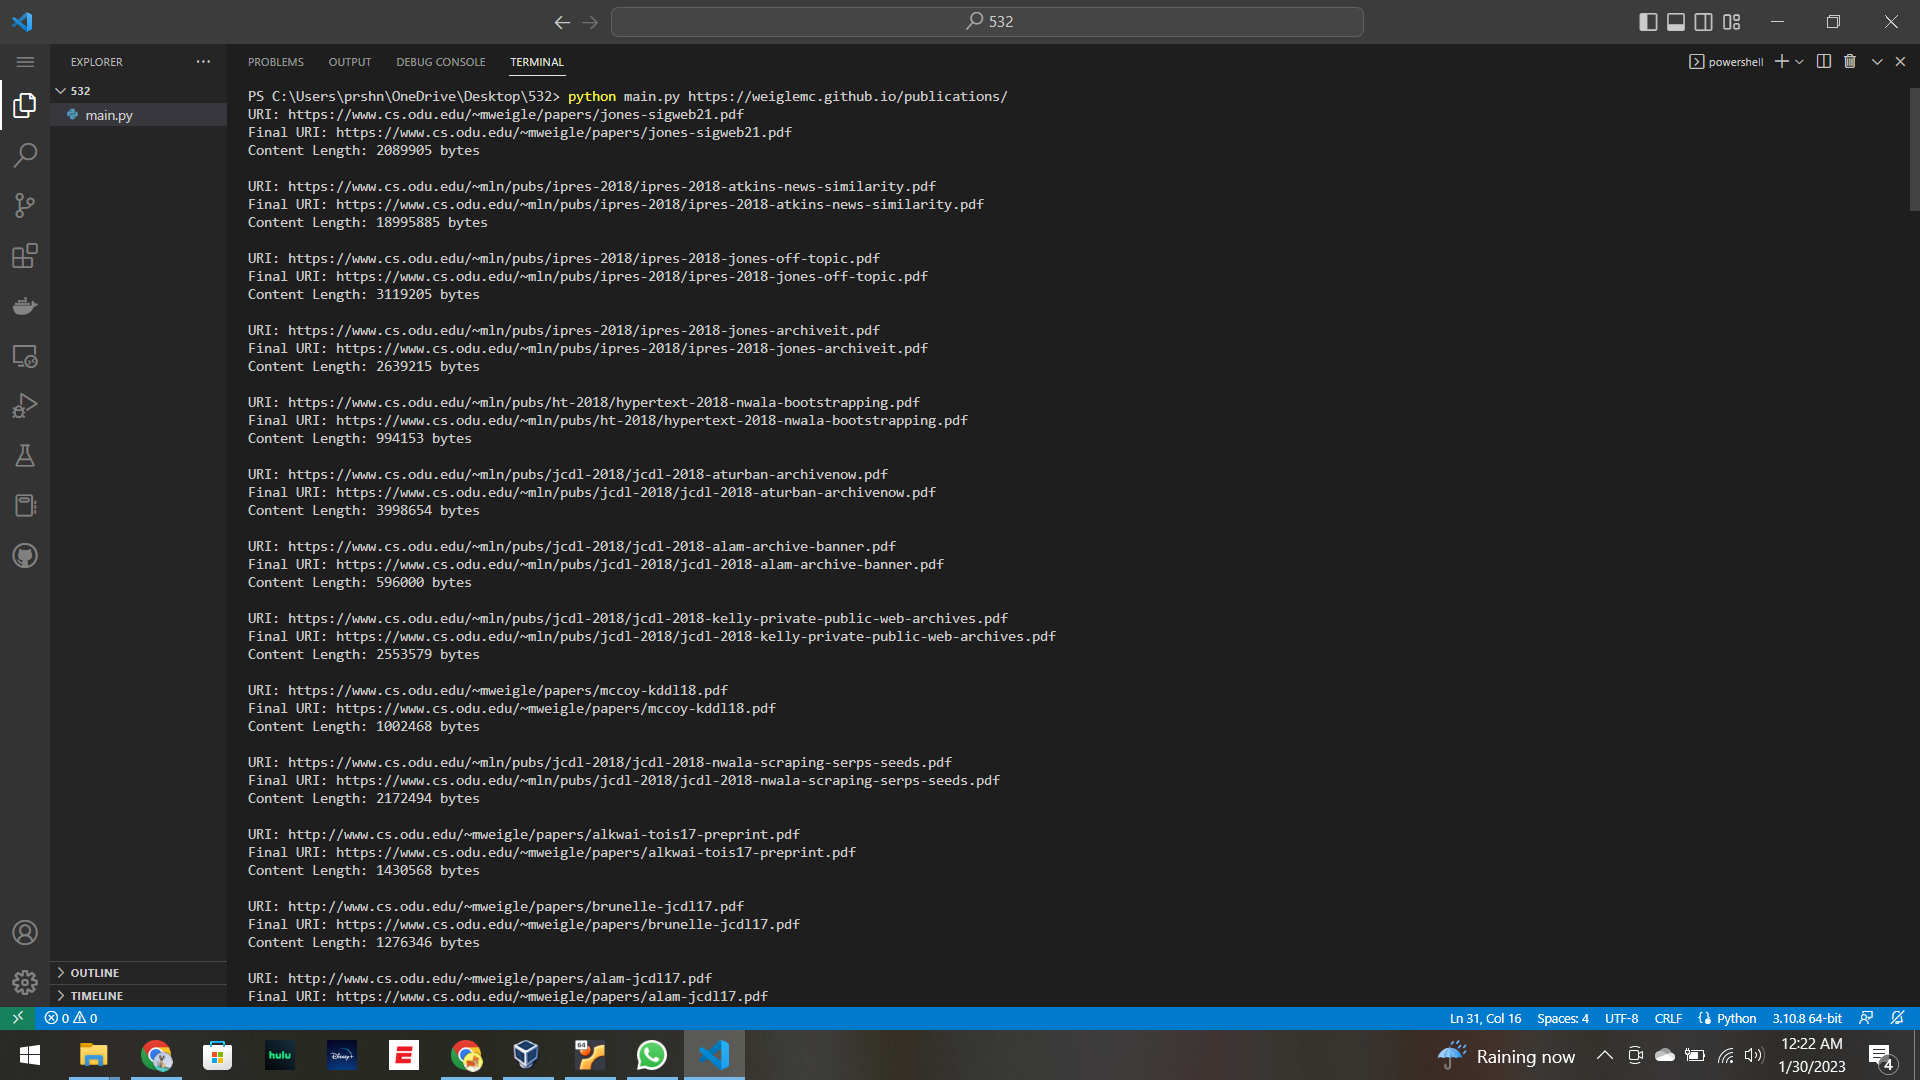
\includegraphics[trim=0 0 0 0, clip, width=\textwidth,height=10cm] {Q3b.png}
    \caption{PDF:2}
    \label{fig:Q3b}
\end{figure}

\begin{figure}[h!]
    \centering
    % trim and clip are used to crop the image, trim=left bottom right top
    % width sets max width, height will be scaled appropriately
    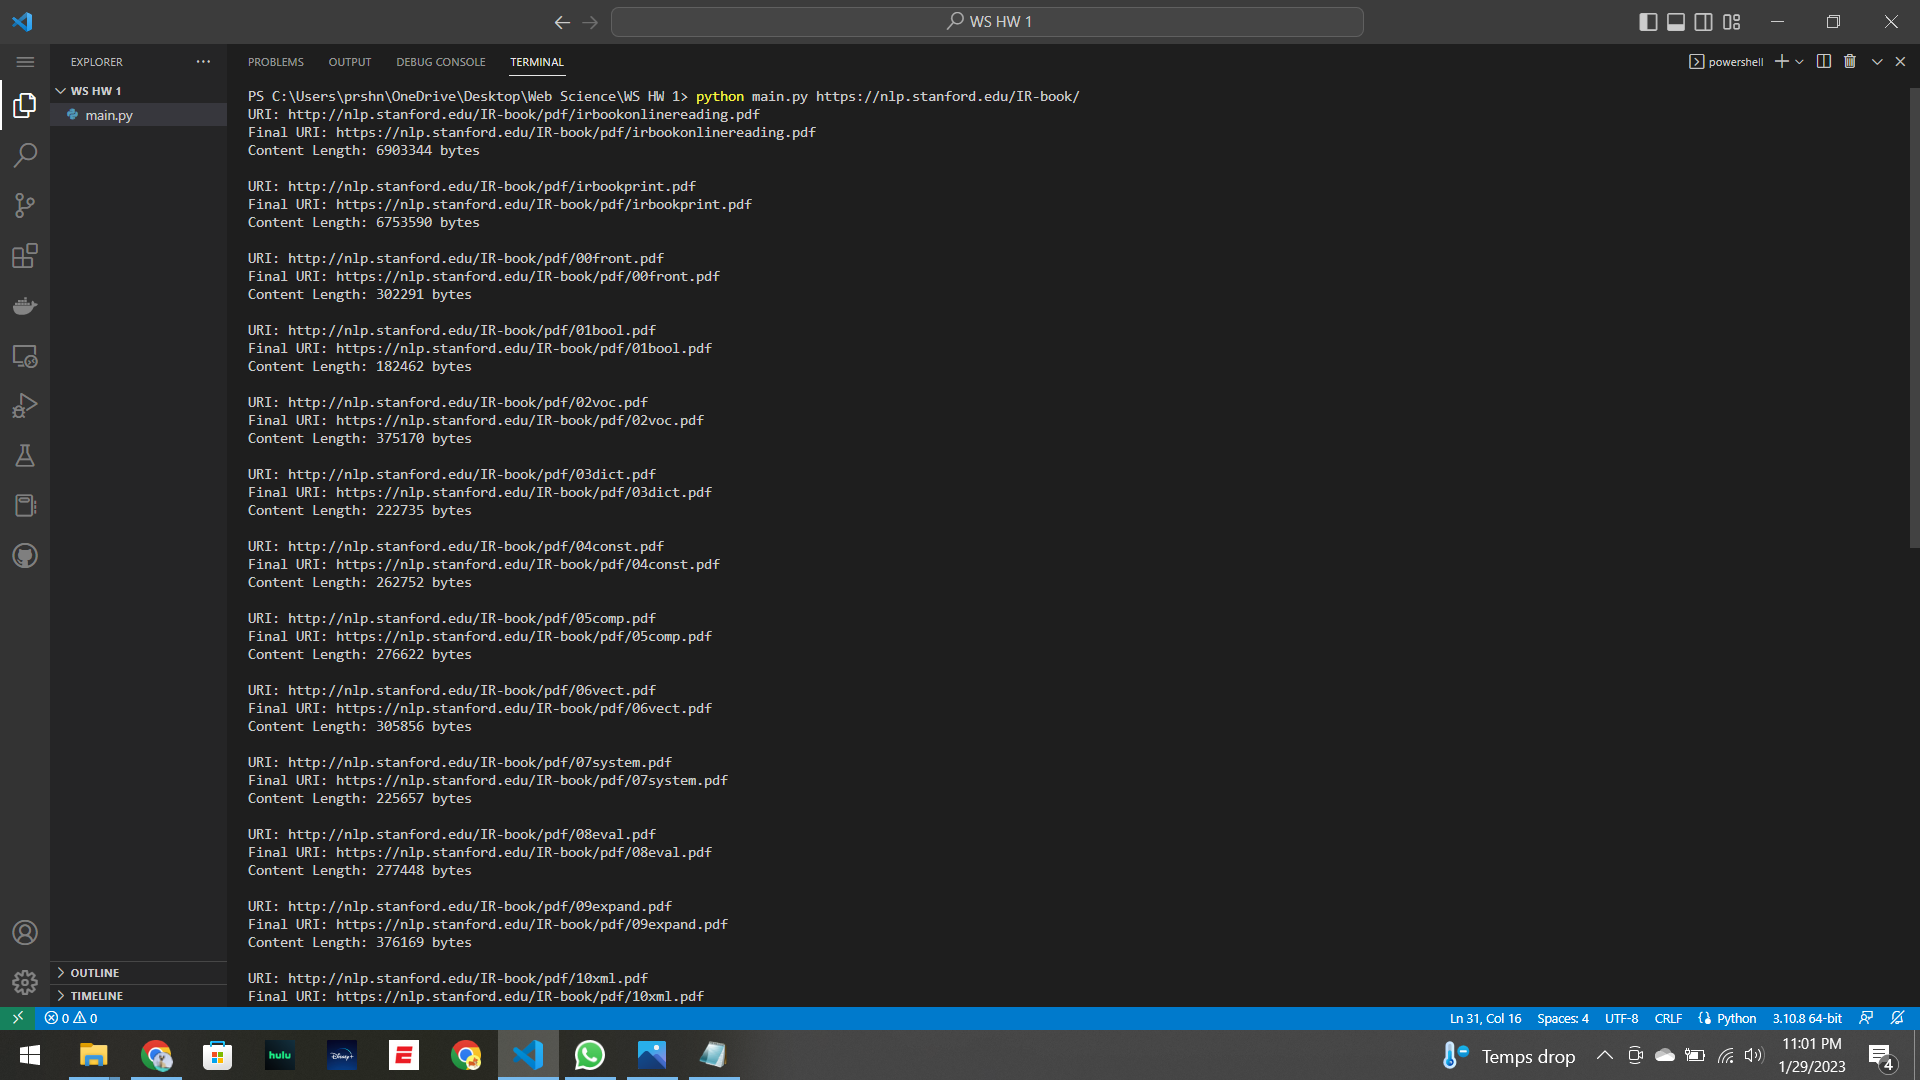
\includegraphics[trim=0 0 0 0, clip, width=\textwidth,height=10cm] {Q3c.png}
    \caption{PDF:3}
    \label{fig:Q3c}
\end{figure}
%Importing code from file
\lstinputlisting[language=Python, caption=Python sample code loaded from file, label=lst:import]{main.py}


\subsection*{Discussion}

\section*{References}

\emph{Every report must list the references that you consulted while completing the assignment. If you consulted a webpage, you must include the URL.}
\section*{References}

\begin{itemize}
    \item {Reference 1, \url{https://docs.python-requests.org/en/v0.8.4/api/}}
    \item {Reference 2, \url{https://developers.google.com/edu/python/regular-expressions}}
\end{itemize}


\end{document}